%--------------------------------------------------------------------------
\chapter{System Analysis and Design using UML}
%
The {\em Unified Modeling Language} (UML) is a general-purpose, developmental,
modeling language in the field of software engineering that is
intended to provide a standard way to visualize the design of a system:
\begin{quote}
The Unified Modeling Language (TM)
 -- UML -- is OMG's most-used specification, and
the way the world models not only application structure, behavior, and
architecture, but also business process and data structure.
\end{quote}

Likewise building plans are created in many other areas, e.g.
architects, machine design, electronic circuits, plans are
also needed for the design and implementation of software
systems.

%Analog zu den Bauplänen, die für Architekten, Maschinenkonstrukteure
%und Elektroniker unabdingbar und selbstverständlich sind,
%hat sie den Anspruch (oder vielmehr das Ziel) solche
%Systeme generell, vollständig und eindeutig zu beschreiben.

\ifslides
\newslide
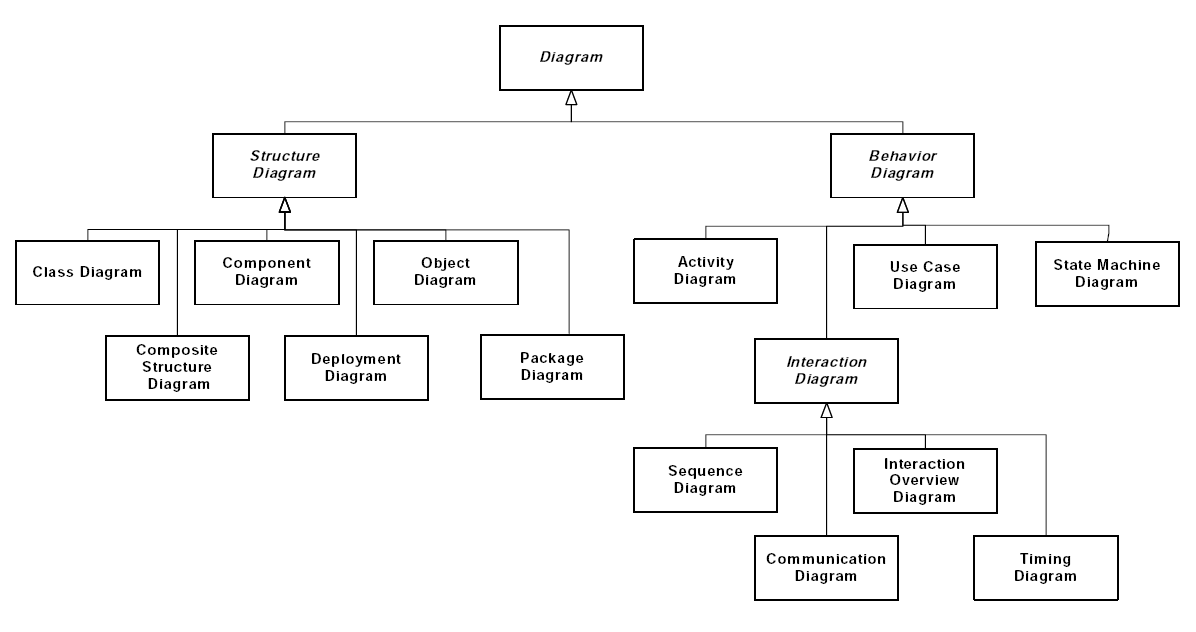
\includegraphics[width=\linewidth]{uml/img/uml-diagrams}
\newslide
\else
UML contains diagrams which could be used for all
areas in the design of a software system.
%Die UML umfasst spezielle Diagramme für
%die Darstellung der verschiedenen Aspekte
%eines Softwaresystems:

\begin{figure}[H]
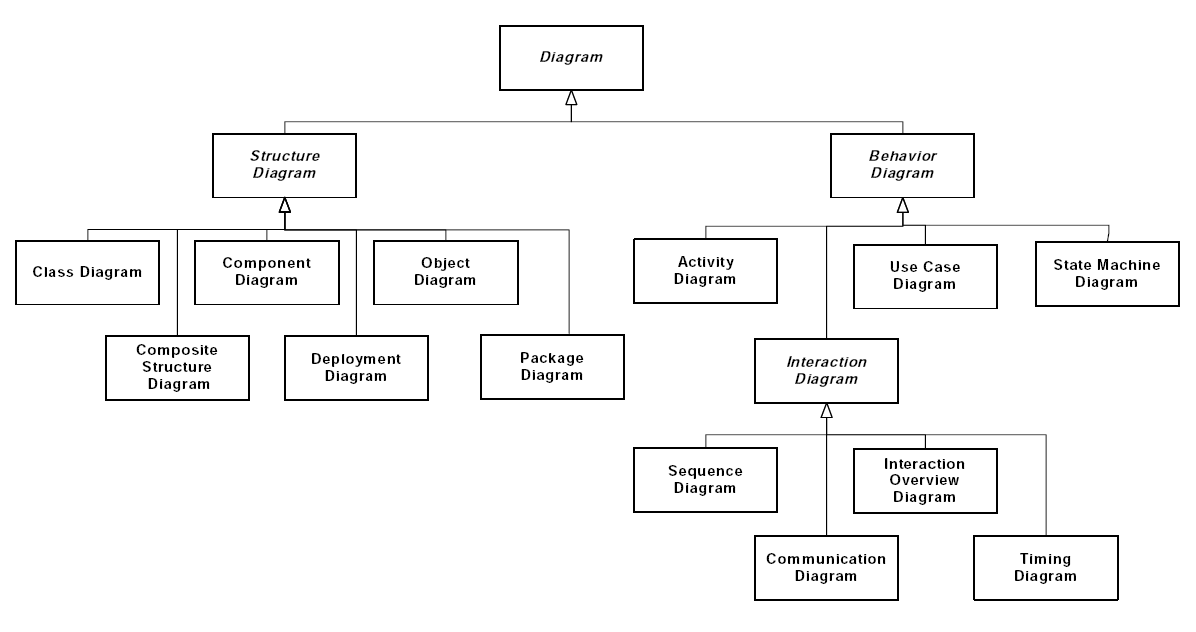
\includegraphics[width=\linewidth]{uml/img/uml-diagrams}
\caption{The Diagrams of UML 2 (Source: OMG)}
\end{figure}
\fi

Für den vereinfachten Austausch der UML-Modelle zwischen
Entwicklungswerkzeugen verschiedener Hersteller wird von OMG auch das
Datenformat {\em XML Metadata Interchange (XMI)} definiert.

%Dazu wird in der Regel ein
% formales Modell erstellt, das die essentiellen Aspekte
%des Systems beschreibt resp. spezifiziert.
\newpage
The current UML standards call for 13 different types of diagrams:
\begin{description}
\item[Structural UML diagrams:] Structure diagrams emphasize the things that
must be present in the system being modeled:
  \begin{description}
  \item[Class Diagram:] Class diagrams are the backbone of almost
  every object-oriented method, including UML. They describe the
  static structure of a system.
  \item[Package Diagram:] Package diagrams are a subset of class
  diagrams, but developers sometimes treat them as a separate
  technique. Package diagrams organize elements of a system into
  related groups to minimize dependencies between packages.
  \item[Component Diagram:] Component diagrams describe the
  organization of physical software components, including
  source code, run-time (binary) code, and executables.
  \item[Deployment Diagram:] Deployment diagrams depict
  the physical resources in a system, including nodes,
  components, and connections.
  \end{description}
\item[Behavioral UML diagrams:] Behavior diagrams emphasize what must
happen in the system being modeled:
  \begin{description}
  \item[Use-Case Diagram:] Use case diagrams model the functionality
  of a system using actors and use cases.
  \item[State-Transition Diagram:] State-Transition diagrams,
  now known as state machine diagrams and state diagrams describe
  the dynamic behavior of a system in response to external stimuli.
  State diagrams are especially useful in modeling reactive objects
  whose states are triggered by specific events.
  \item[Activity Diagram:] Activity diagrams illustrate the dynamic
  nature of a system by modeling the flow of control from activity
  to activity. An activity represents an operation on some class in
  the system that results in a change in the state of the system.
  Typically, activity diagrams are used to model workflow or business
  processes and internal operation.
  \item[Interaction diagram:] Interaction diagrams describe interactions
  among classes in terms
  of an exchange of messages over time.
  \item[Timing Diagram:] A timing diagram is a type of behavioral or
  interaction UML diagram that focuses on processes that take place
  during a specific period of time. They're a special instance of a
  sequence diagram, except time is shown to increase from left to right
  instead of top down.
  \end{description}
\end{description}
\newpage
%--------------------------------------------------------------------------
%\subsection{UML-Diagramme}
\section{Class Diagram}
The class diagram is the main building block of object-oriented
modeling. It is used for general conceptual modeling of the
structure of the application, and for detailed modeling translating
the models into programming code. Class diagrams can also be used for
data modeling. The classes in a class diagram represent both the
main elements, interactions in the application, and the classes to be
programmed.

\ifslides
\newpage
\paragraph{Class}\\[2ex]
\begin{minipage}[c]{0.45\linewidth}
\else
\paragraph{Class}\mbox{} \\
\begin{minipage}[c]{0.5\linewidth}
\fi
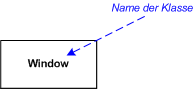
\includegraphics[width=\linewidth]{uml/img/Class-1}\\

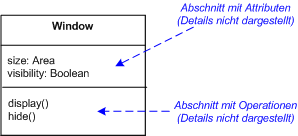
\includegraphics[width=\linewidth]{uml/img/Class-2}\\

%\includegraphics[width=3cm]{uml/img/Class-3}\\
%
{\footnotesize Source: wikipedia}
\end{minipage}
\hfill
\begin{minipage}[c]{0.45\linewidth}
A class contains a name, attributes and methods. Attributes and
methods could be hidden if they do not cover an important part in
the system design.
\end{minipage}
%
\paragraph{Interface}\mbox{} \\
\begin{minipage}[c]{0.28\linewidth}
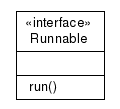
\includegraphics[width=3cm]{uml/img/interface}
\end{minipage}
\begin{minipage}[c]{0.7\linewidth}

Interface are similar to abstract classes.
It is a collection of abstract methods.
A class implements an interface, thereby inheriting
the abstract methods of the interface.
Along with abstract methods, an interface may also
contain constants, default methods, static methods,
and nested types.
\end{minipage}
%
\ifslides
\newpage
\fi
\paragraph{Abstract class}\mbox{} \\
\begin{minipage}[c]{0.28\linewidth}
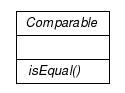
\includegraphics[width=3cm]{uml/img/abstract}
\end{minipage}
\begin{minipage}[c]{0.7\linewidth}
An abstract class is a class that is declared abstract. It
may or may not include abstract methods.
Abstract classes cannot be instantiated, but they can be subclassed.
\end{minipage}
%
\newpage
%
\paragraph{Attributes and Methods}\mbox{} \\
\begin{minipage}{0.3\linewidth}
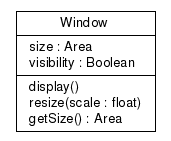
\includegraphics[width=\linewidth]{uml/img/window}
\end{minipage}
\hfill
\begin{minipage}{0.65\linewidth}

An \structure{attribute} is an individual thing that differentiate one object from
another and determine the appearance, state, or other qualities of that object.
Each object for a class has the given set of attributes with
own values.

A \structure{class attribute} is an attribute which exists only once
for all objects. All objects of a given class share the same attribute.
Class attributes are underlined.

A \structure{method} is a set of statements to perform an operation.
Sometimes, a method is also called member function.

A \structure{class method} is an operation which does not depend on any object
of that class. This method could also be called if there is no object of the
class (e.g. utility method), therefore a class method could not access any
attributes (expect class attributes).
\end{minipage}

%Eine abstrakte Operation ist eine Operation, f\"ur die nur eine Signatur,
%jedoch keine Anweisungsfolge definiert ist, d.h. die Operation ist definiert,
%aber noch nicht implementiert. Sie wird in einer abgeleiteten Klasse
%implementiert. Abstrakte Operationen werden \"ublicherweise durch
%Kursivschrift gekennzeichnet.
\ifslides
\newpage
\fi
%
\paragraph{Visibility}\mbox{} \\
\begin{minipage}[c]{0.4\linewidth}
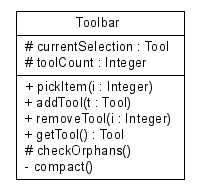
\includegraphics[width=0.85\linewidth]{uml/img/visibility}
\end{minipage}
\begin{minipage}[c]{0.58\linewidth}
There are 3 different types of visibility for attributes and methods:

\begin{description}
\item [-- Private] only visible within the class

\item [\# Protected] visible in the class itself and all inherited classes

\item [+ Public] visible from everywhere, no protection.
\end{description}
\end{minipage}

%\ifslides
\newpage
%\fi
\paragraph{Inheritance} (generalization)\\[2ex]
\begin{minipage}[c]{0.5\linewidth}
\ifslides
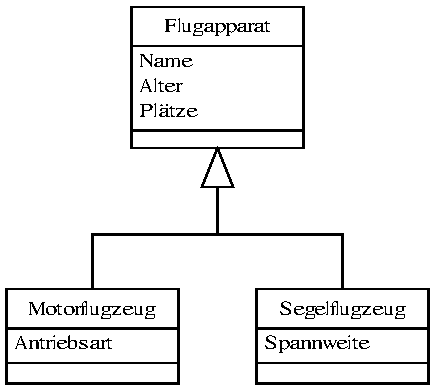
\includegraphics[width=\linewidth]{uml/img/Vererbung}
\else
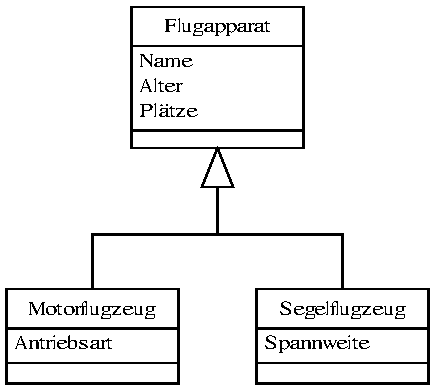
\includegraphics[width=\linewidth]{uml/img/Vererbung}
\fi
\end{minipage}
\begin{minipage}[c]{0.45\linewidth}

In object-oriented programming, inheritance is the mechanism of basing an
class upon another class, retaining similar implementation. Also defined as
deriving new classes (sub classes) from existing ones (super class)
and forming them into a hierarchy of classes. Aan object created through
inheritance acquires all the properties and behaviors of the parent
object (except: constructors, and some other language specific constructs).
Inheritance allows programmers to create classes
that are built upon existing classes, to specify a new implementation while
maintaining the same behaviors (realizing an interface), to reuse code and to
independently extend original software via public classes and interfaces.
\end{minipage}
%
\newpage
\paragraph{Association}\mbox{} \\
\begin{minipage}[c]{0.28\linewidth}
\ifslides
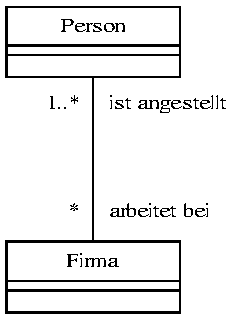
\includegraphics[width=3.2cm]{uml/img/Assoziation}
\else
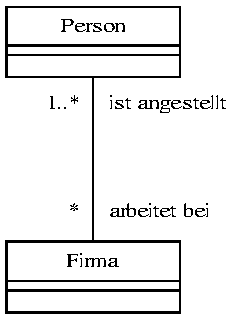
\includegraphics[width=3.7cm]{uml/img/Assoziation}
\fi
\end{minipage}
\begin{minipage}[c]{0.7\linewidth}
An \structure{association} defines a relationship between classes of
objects that allows one object instance to cause another to perform an action
on its behalf. This relationship is structural, because it specifies that
objects of one kind are connected to objects of another and does not
represent behaviour.
\end{minipage}
%
\ifslides
\newpage
\fi
\paragraph{Aggregation}\mbox{} \\
\begin{minipage}[c]{0.28\linewidth}
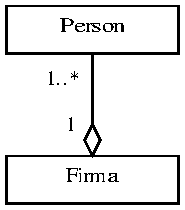
\includegraphics[width=3cm]{uml/img/Aggregation}
\end{minipage}
\begin{minipage}[c]{0.7\linewidth}
Inheritance is a \verb|"|is-a\verb|"| relation (e.g. a dog (sub class) is a animal
(super class)). An \structure{aggregation} contains a whole/part
relationship (\verb|"|has-a\verb|"|). A synonym for this is \verb|"|part-of\verb|"|.
\end{minipage}
%
\ifslides
\newpage
\fi
\paragraph{Composition}\mbox{} \\
\begin{minipage}[c]{0.28\linewidth}
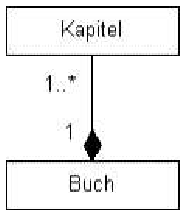
\includegraphics[width=3cm]{uml/img/Komposition}
\end{minipage}
\begin{minipage}[c]{0.7\linewidth}
A \structure{composition} is a restricted form of Aggregation in which two
entities are highly dependent on each other. When there is a composition
between two entities, the composed object cannot exist without the other entity.
\end{minipage}
%
\ifslides
\newpage
\fi
\paragraph{Comment} (note)\\[2ex]
\begin{minipage}[c]{0.3\linewidth}
\ifslides
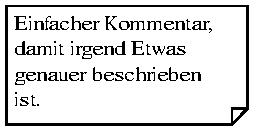
\includegraphics[width=3.5cm]{uml/img/Kommentar1}
\else
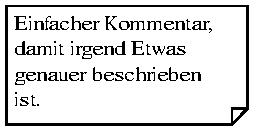
\includegraphics[width=4.3cm]{uml/img/Kommentar1}
\fi
\end{minipage}
\begin{minipage}[c]{0.69\linewidth}
Comments could be added for additional clarification or description.
\end{minipage}
%
\newpage
\ifslides
\paragraph{Beispiel}\ \\
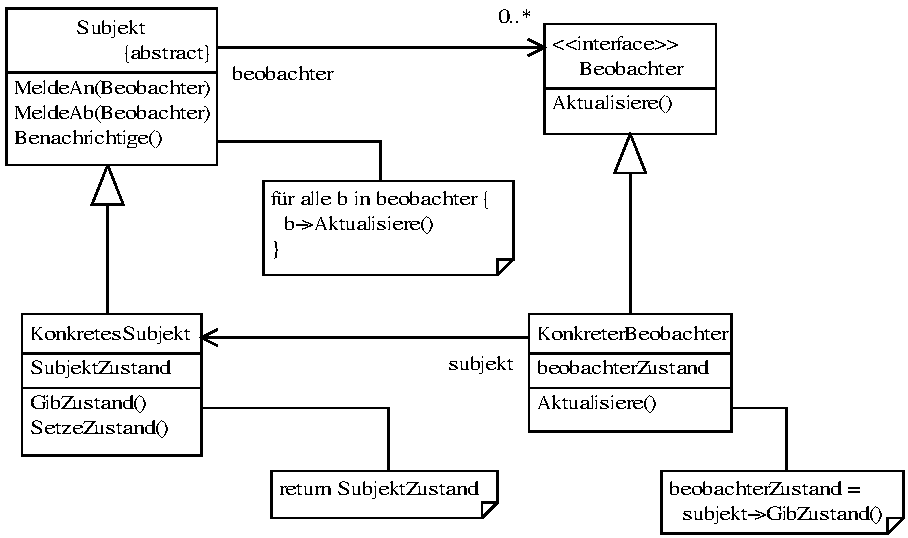
\includegraphics[width=0.9\linewidth]{uml/img/Beobachter}
\else
\paragraph{Beispiel}
Ein Objekt soll in der Lage sein, andere Objekte zu benachrichtigen,
ohne Annahmen dar\"uber zu treffen, wer die anderen Objekte sind.
Mit anderen Worten: gesucht ist eine Struktur mit
 möglichst lose gekoppelten Objekten.
Die L\"osung dieses Problems ist unter dem Begriff
Beobachter (Observer) bekannt.
%
\begin{figure}[H]
\begin{center}
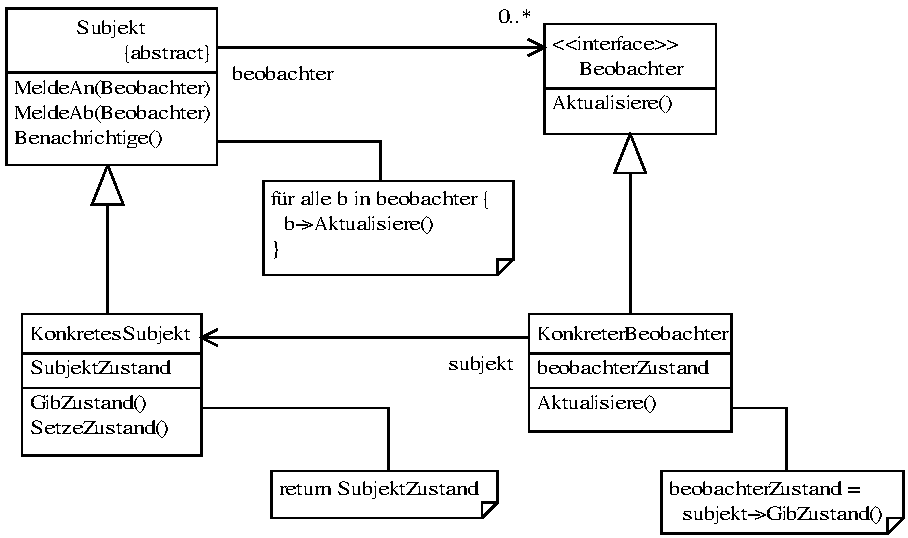
\includegraphics[width=\linewidth]{uml/img/Beobachter}
\caption{Entwurfsmuster Beobachter}
\end{center}
\end{figure}
\fi
%
%\begin{center}
%\ifslides
%\includegraphics[width=0.4\linewidth]{uml/xfig/uml-classdiagram}
%\else
%\includegraphics[width=0.7\linewidth]{uml/xfig/uml-classdiagram}
%\fi
%\end{center}
\ifslides
\newpage
\fi
\underline{Vorgehen}
\begin{enumerate}
\item Klassen und Beziehungen identifizieren,
\item die relevanten Attribute und Methoden hinzuf\"ugen,
\item generalisieren durch Vererbung,
\item die Klassen in Kategorien (Module) gruppieren
\end{enumerate}
%--------------------------------------------------------------------------
\newpage
\subsection{The Creation of Class Diagrams}
\underline{1. Schritt: Identifizieren von Klassen und deren Beziehungen}\\[2ex]
Ausgangspunkt ist den meisten F\"allen eine verbale Beschreibung des
Problembereichs im Vokabular des Anwenders. Eine g\"angige, wenn
auch zum Teil kritisierte, Methode
zur Identifizierung der Klassen (und Objekte) basiert auf einer Textanalyse,
bei der die Substantive als m\"ogliche Kandidaten dienen:\\[2ex]
\begin{tabularx}{\linewidth}{l|X}
Personen, Rollen & Lieferant, Kunde, Mitarbeiter, Student, Dozent \\
Dinge, Ger\"ate  & Beh\"alter, Tank, Regler, Pumpe, Zeitgeber, Schalter,
            Messger\"at, Sensor, Filter, Anzeige\\
Abstraktionen & Stack, Array, Tabelle, Sequenz, Menge, Figur, Dreieck, Linie,
    Datei, Baustein, Element\\
%%\item[Orte]
Beschreibungen, Dokumente & Rezeptur, Produkt, Konto\\
Ereignisse, Vorg\"ange & Prozess, Simulation, Steuerung, Nachricht\\
Interaktionen& Bestellung, Kaufvertrag, Buchung, Reservation,
Anmeldung, Auftrag
%%\item[Externe Systeme]
%%\item[Organisationseinheiten]
\end{tabularx}

In der Regel findet man in einer ersten Analyse des Problembereichs
mehr Klassen, als man wirklich ben\"otigt. Auf weiter zu verwendende Klassen
m\"ussen die folgenden Aussagen zutreffen:
\begin{enumerate}
\item Ihr Name ist eindeutig, d.h. kein Synonym einer bereits
 ausgew\"ahlten Klasse.
\item Sie enth\"alt Informationen (Attribute), die innerhalb
  des Systems gespeichert werden sollen.
\item Sie stellt system-relevante Operationen zur Verf\"ugung (mehr als
   nur Setzen und Abfragen).
\end{enumerate}
Beziehungen zwischen den Objekten entsprechen physischen oder
logischen Verkn\"upfungen mit zugeh\"origen Kardinalit\"aten
analog den Relationen zwischen Entit\"aten:
\begin{itemize}
\item Assoziation: semantische Verkn\"upfung
\item Aggregation: ``hat-ein''-Verkn\"upfung
\item Verwendung: Nutzungs-Verkn\"upfung
\item Vererbung: ``ist-ein''-Verkn\"upfung
\end{itemize}
\newpage
%--------------------------------------------------------------------------
%{\bfseries Beispiel:} Es soll ein einfaches
%Zeichnungsprogramm entwickelt werden, mit welchem der Anwender
%verschiedene Figuren (Linien, Rechtecke) mit dem Mauszeiger
%erzeugen und in einer
%Zeichenfl\"ache darstellen kann.
%Eine Reihe in senkrechter Kolonne angeordneter und
%gegenseitig sich ausschliessender
%Kontrollkn\"opfe, die sich am rechten (oder linken) Rand der
%Zeichenfl\"ache befindet, erlaubt die Auswahl des zu zeichnenden Figurentyps.
%Mit einer weiteren solchen Reihe kann die Farbe gew\"ahlt werden.
%Schliesslich gibt es noch Druckkn\"opfe zum L\"oschen oder Verlassen des
%Programms.
%\newpage
%--------------------------------------------------------------------------
%\subsection*{Objektorientierte Analyse (Object-Oriented Analysis)}
{\bfseries Beispiel:} Klassendiagramm eines bekannten Spiels:\\[1.5ex]
%%
\begin{center}
\ifslides
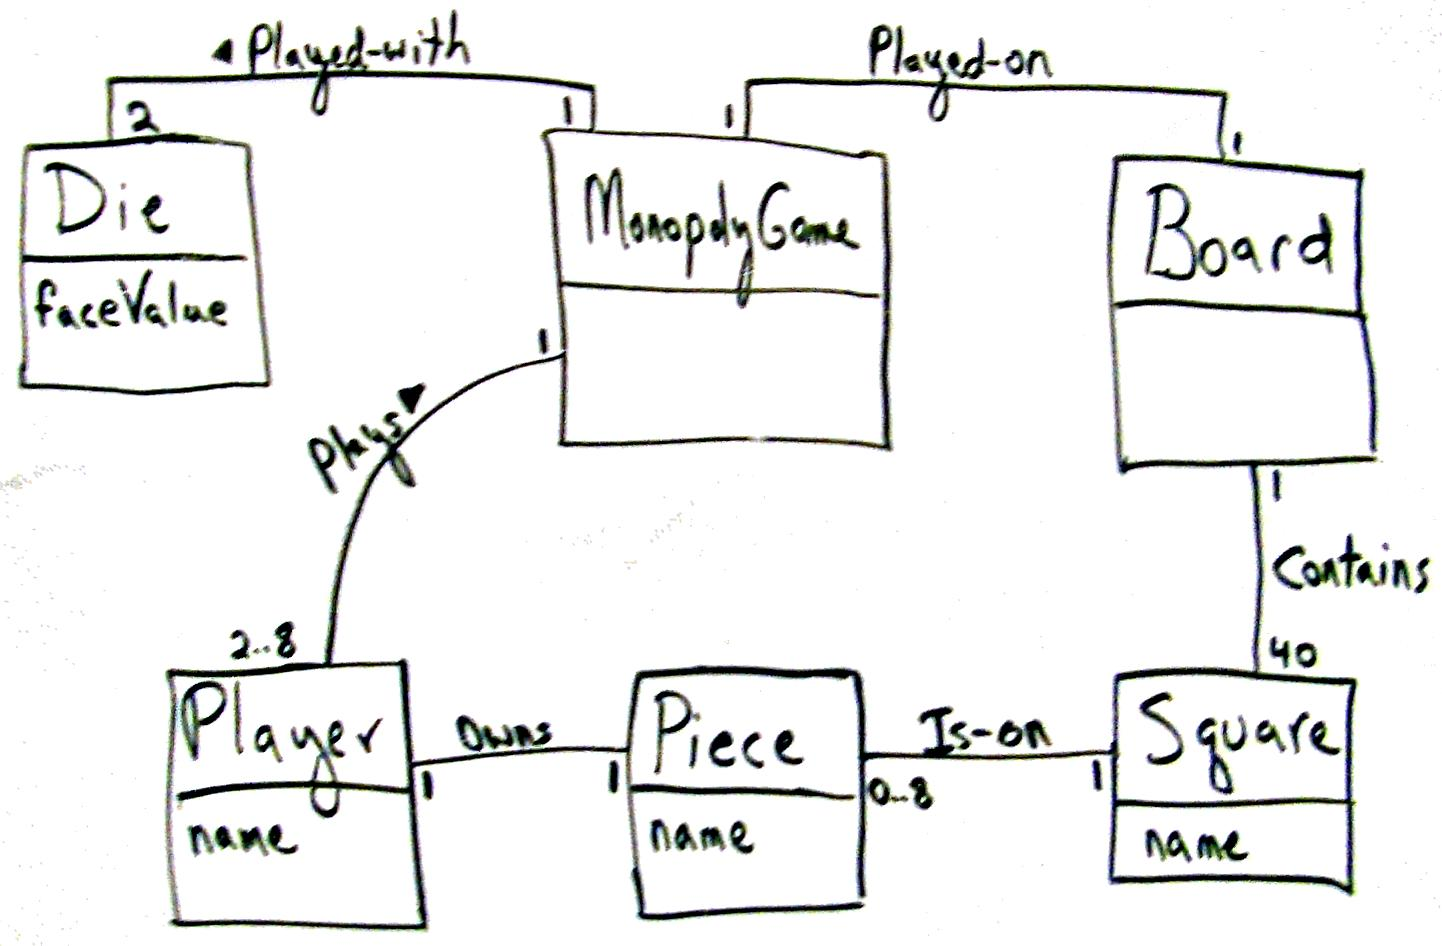
\includegraphics[width=0.77\linewidth]{uml/img/monopoly}
\else
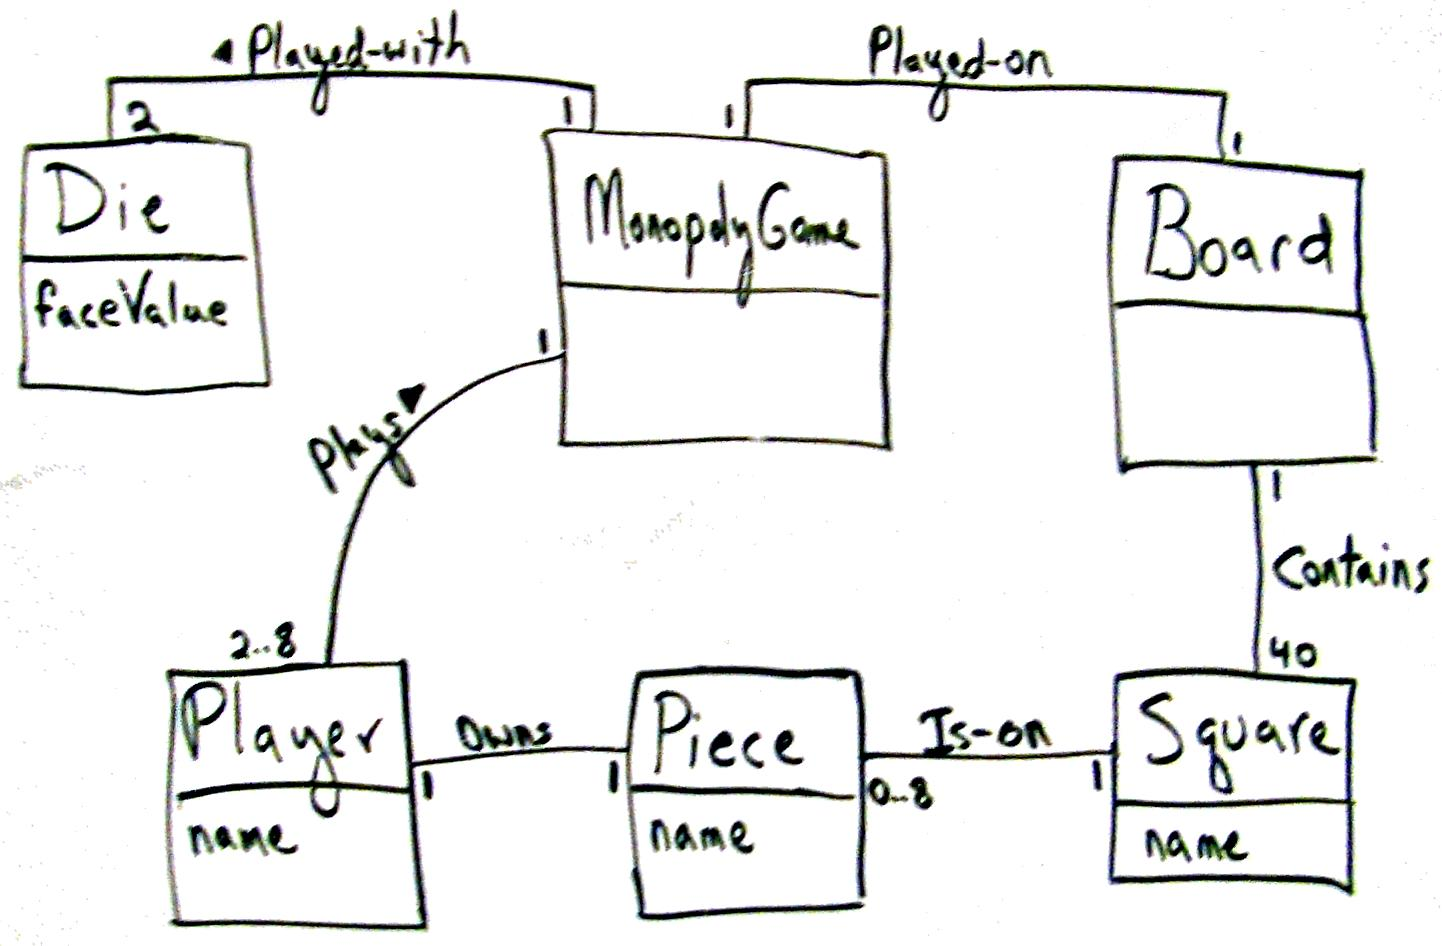
\includegraphics[width=0.9\linewidth]{uml/img/monopoly}
\fi
\end{center}
\ifslides
\else
{\footnotesize Source: Craig Larman}\\[2ex]
\fi
%--------------------------------------------------------------------------
%\subsection*{Klassendiagramm}
\underline{2. Schritt: Hinzuf\"ugen der relevanten Attribute und Methoden}
\begin{itemize}
\item Attribute sind die Eigenschaften der Objekte:
\begin{enumerate}
\item Wie wird das Objekt allgemein beschrieben?
\item Wie wird das Objekt im Problembereich beschrieben?
\item Können zusammengehörende Attribute zu einer Gruppe
  zusammengefasst werden?
 (Bsp: Vorname, Nachname, Anrede ergibt Name)
\end{enumerate}
\item Methoden sind die Dienste, die ein Objekt bereitstellt:
\begin{enumerate}
\item Berechnungen
\item \"Uberwachung
\item Kommunikation
\end{enumerate}
aus Gründen der \"Ubersichtlichkeit sollen nur explizite und
keine impliziten Methoden im Objektmodell dargestellt werden.
Implizite Methoden sind: Konstruktorfunktionen, Zugriffsfunktionen zu den
  Attributen, Verbindungsfunktionen zum Setzen und L\"osen von Verbindungen.
\end{itemize}
\newpage
\underline{3. Schritt: Generalisieren durch Vererbung}\\[2ex]
Durch eine Vererbungsstruktur werden Klassen
die
\begin{itemize}
\item Spezialfälle einer andern Klasse sind oder
\item gemeinsame Attribute mit andern Klassen haben
\end{itemize}
in einer gemeinsamen Basisklasse zusammengefasst.\\[3ex]
\underline{4. Schritt: Gruppierung der Klassen in Kategorien}
\begin{itemize}
\item Jede Klasse ist Teil genau einer Kategorie.
\item Die Kopplung zwischen Klassen unterschiedlicher Kategorien ist minimal.
\end{itemize}
\ifslides
\newpage
\fi
%--------------------------------------------------------------------------
\section{Interaction Diagrams}
An \structure{interaction diagram} visualizes the interactions between
objects.

One interaction diagram normally demonstrates the behavior of one
single use case. The diagram shows a number of objects as well as
all messages which are exchanged between these objects.

There are two types of interaction diagrams:
sequence diagram and collaboration diagram

%
\paragraph{Sequence diagram}\mbox{} \\
A \structure{sequence diagram} shows object interactions arranged in time sequence.
It depicts the objects and classes involved in the scenario and the sequence
of messages exchanged between the objects needed to carry out the
functionality of the scenario.

A sequence diagram shows, as parallel vertical lines (lifelines),
different processes or objects that live simultaneously, and, as
horizontal arrows, the messages exchanged between them, in the order in
which they occur. This allows the specification of simple runtime scenarios
in a graphical manner.

%Um zu zeigen, dass ein Objekt aktiv ist, kann man einen
%\emph{Aktivierungskasten} (engl.
%activitation box) hinzuf\"ugen. Man kann
%Aktivierungsk\"asten weglassen, wodurch die Diagramme
%einfacher zu zeichnen, jedoch auch schwieriger zu verstehen werden.

%Zwei Anteile der Steuerinformationen k\"onnen besonders n\"utzlich sein.
%
%Erstens kann eine \emph{Einschr\"ankung} angeben, wann
%eine Nachricht gesendet wird. Die Nachricht
%wird nur gesendet, wenn die Einschr\"ankung wahr ist.
%
%Die zweite n\"utzliche Steuermarkierung ist die Iterationsmarkierung.
%Sie zeigt an, dass eine
%Nachricht mehrfach an viele Empf\"angerobjekte gesendet wird. Woraus
%sich die Iteration ergibt,
%kann man in eckigen Klammern darstellen
%(wie z.B. *[f\"ur alle
%Auftragspositionen]).

%Das Löschen eines Objekts wird mit einem grossen \textbf{X} markiert.
%\ifslides
%\else
%
%Auftragsbearbeitung als Sequenzdiagramm.
%\fi
%
\begin{figure}[H]
\begin{center}
\ifslides
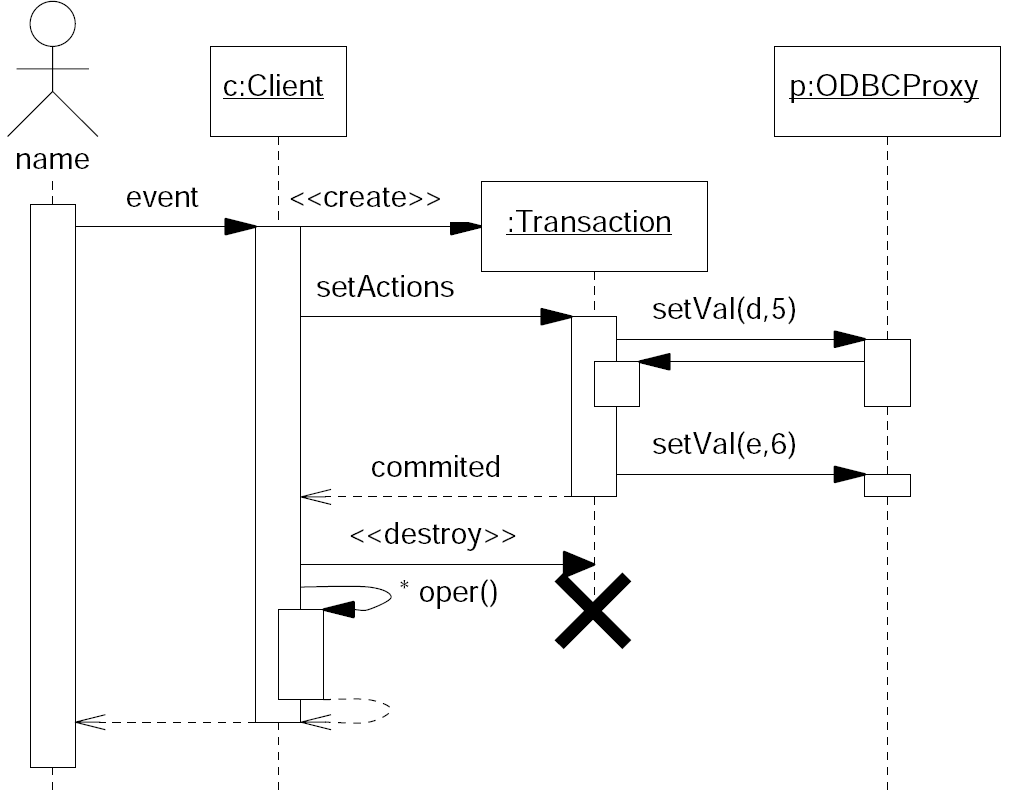
\includegraphics[width=0.7\linewidth]{uml/img/uml-sequence-diagram}
\else
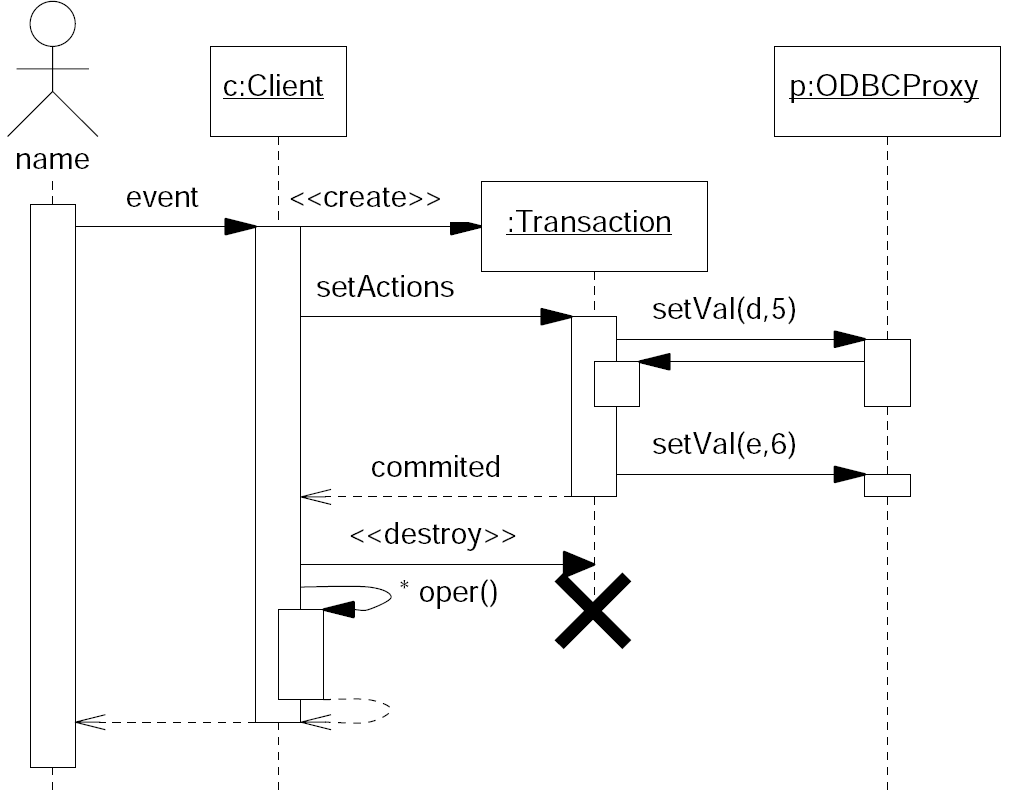
\includegraphics[width=\linewidth]{uml/img/uml-sequence-diagram}
\fi
\caption{Sequenzdiagramm}
\label{SEQ}
\end{center}
\end{figure}
\ifslides
\begin{center}
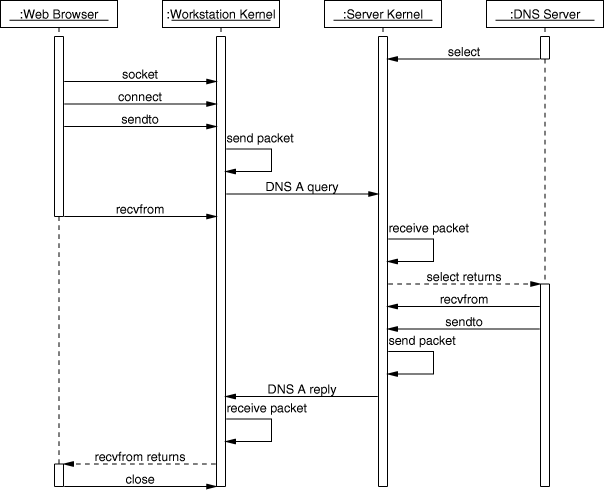
\includegraphics[width=0.75\linewidth]{uml/img/dnsquery}
\end{center}
\else
\begin{figure}[H]
\begin{center}
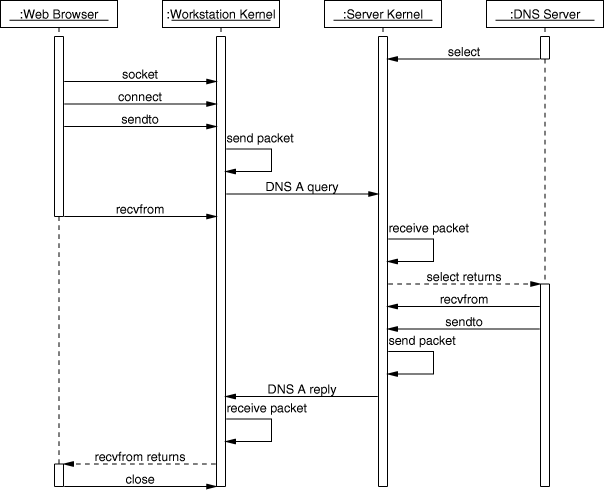
\includegraphics[width=\linewidth]{uml/img/dnsquery}
\caption{Sequenzdiagramm einer DNS-Abfrage (Source: Craig Larmann)}
%\label{SEQ}
\end{center}
\end{figure}
\fi
%
\paragraph{Collaboration diagram}\mbox{} \\
A \structure{collaboration diagram} models the interactions between objects
or parts in terms of sequenced messages. Collaboration diagrams represent
a combination of information taken from Class, Sequence, and Use Case
Diagrams describing both the static structure and dynamic behavior of a system.

However, communication diagrams use the free-form arrangement of objects
and links as used in Object diagrams. In order to maintain the ordering of
messages in such a free-form diagram, messages are labeled with a
chronological number and placed near the link the message is sent over.
Reading a communication diagram involves starting at message 1.0, and
following the messages from object to object.

Communication diagrams show a lot of the same information as sequence
diagrams, but because of how the information is presented, some of it
is easier to find in one diagram than the other. Communication diagrams
show which elements each one interacts with better, but sequence
diagrams show the order in which the interactions take place more clearly.

\ifslides
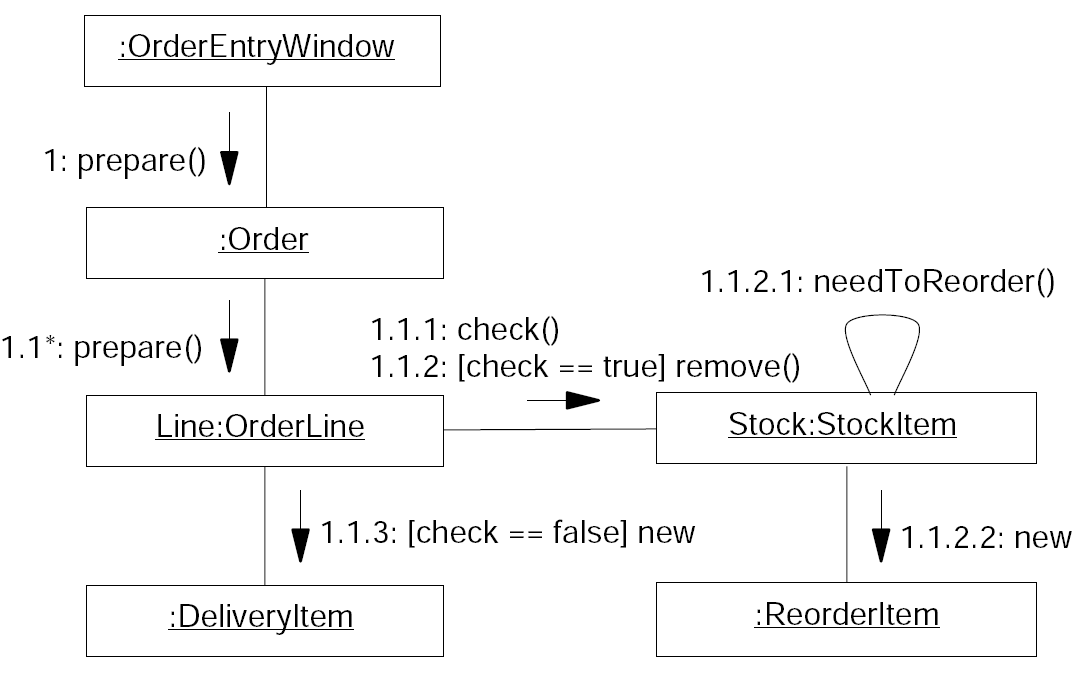
\includegraphics[width=0.9\linewidth]{uml/img/uml-collaboration-diagram}
\else
\paragraph{Beispiel}
%Auftragsbestellung
%
\begin{figure}[H]
\begin{center}
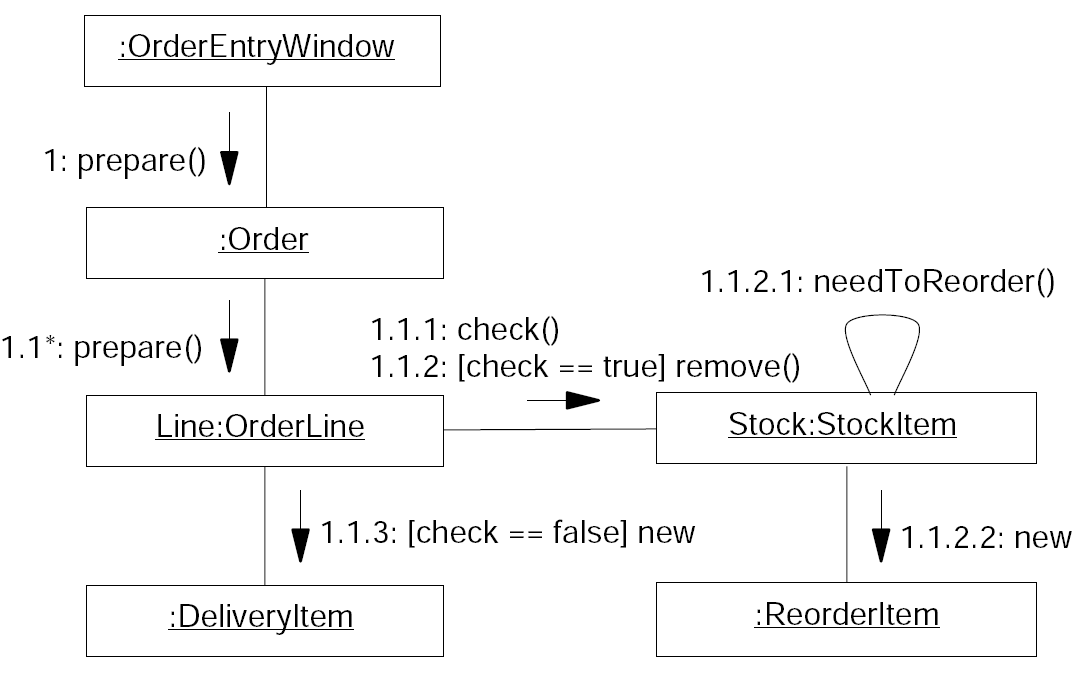
\includegraphics[width=\linewidth]{uml/img/uml-collaboration-diagram}
\caption{Kollaborationsdiagramm}
\label{fig:KOL1}
\end{center}
\end{figure}
%
\fi
%%
\ifslides
\newpage
\fi
\underline{Vorgehen}
\begin{enumerate}
\item Szenarien entwerfen
\item Ereignisse und betroffene Objekte identifizieren
\item Ereignispfad skizzieren
\end{enumerate}
%\newpage
\ifslides
\newpage
\fi
%--------------------------------------------------------------------------
\section{State Transition Diagram}
%%% (Sequence und State-Transition-Diagram)}
State transition diagrams are used to give an abstract description of the behavior of a
system. This behavior is analyzed and represented by a series of events that
can occur in one or more possible states. Hereby each diagram usually
represents objects of a single class and track the different states of its
objects through the system. An object is always in one (and only one) state.
If a event occurs, the state may change.

%
\ifslides
\begin{center}
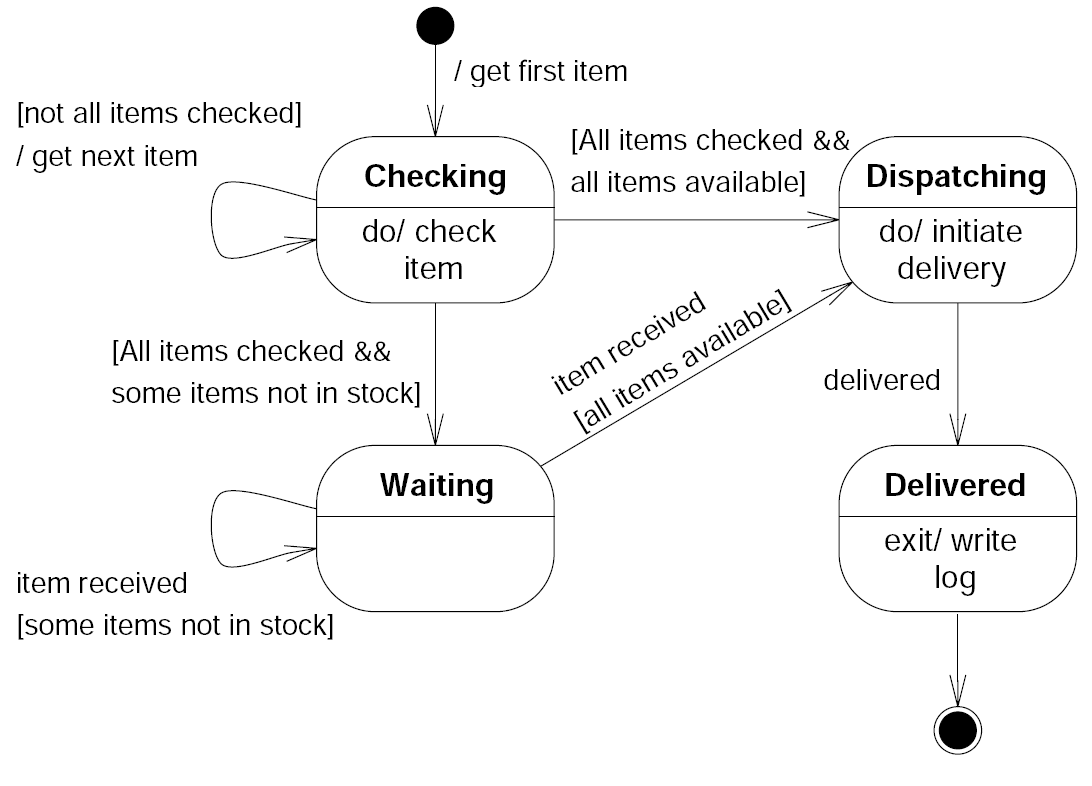
\includegraphics[width=0.8\linewidth]{uml/img/uml-state-diagram}
\end{center}
\else
\newpage
\paragraph{Beispiel}\ \\[2ex]
The following diagram shows the different states for an order (online shop).
\begin{figure}[H]
\begin{center}
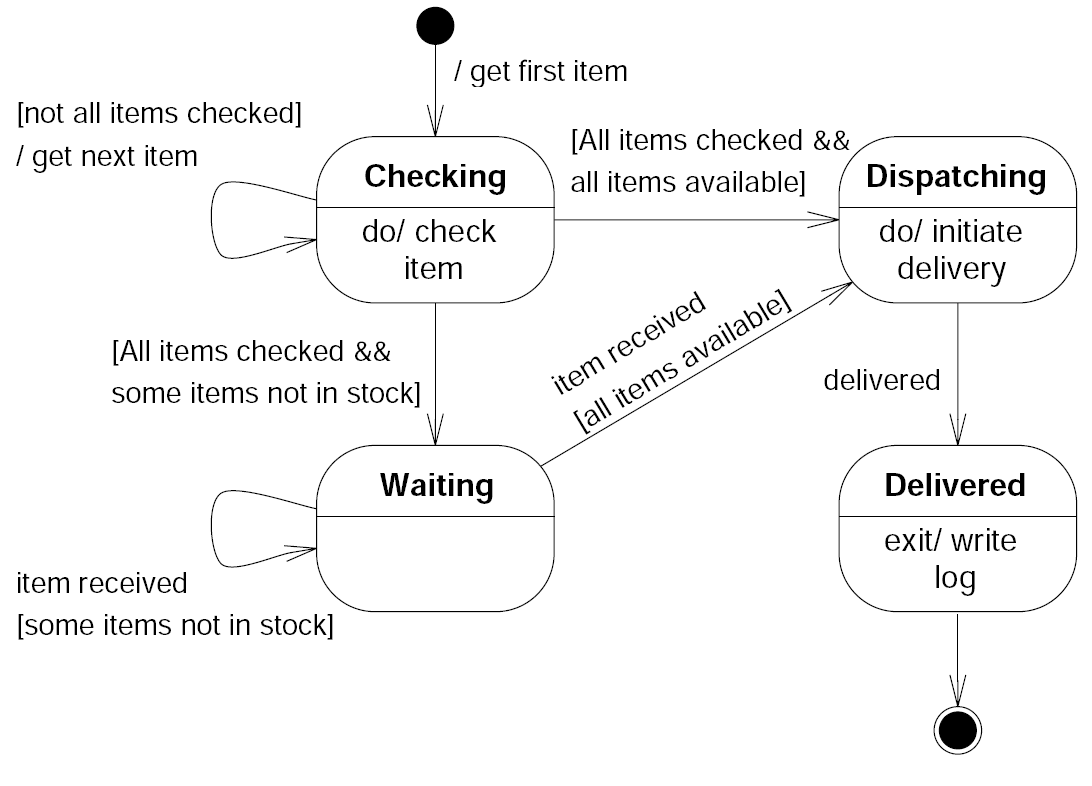
\includegraphics[width=\linewidth]{uml/img/uml-state-diagram}
\caption{Zustandsdiagramm}
\end{center}
\end{figure}
\fi
%
\paragraph{Anfangszustand}\ \\[2ex]
\begin{minipage}[c]{0.1\linewidth}

\includegraphics[width=0.8cm]{uml/img/Anfangszustand}
\end{minipage}
\begin{minipage}[c]{0.89\linewidth}
Jeder Zustandsautomat muss einen Anfangszustand besitzen.
Es handelt sich um einen Pseudozustand, der durch eine
Transition mit einem echten Zustand verbunden ist.
\end{minipage}
%
\paragraph{Endzustand}\ \\[2ex]
\begin{minipage}[c]{0.1\linewidth}

\includegraphics[width=1cm]{uml/img/Endzustand}
\end{minipage}
\begin{minipage}[c]{0.89\linewidth}
Ein Zustandsautomat kann einen Endzustand besitzen.
Im Endzustand (ebenfalls ein Pseudozustand) h\"ort ein Objekt auf zu
existieren.
\end{minipage}
%
\newpage
\paragraph{State}\ \\[2ex]
\begin{minipage}[c]{0.28\linewidth}
\ifslides
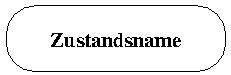
\includegraphics[width=2.8cm]{uml/img/Zustand}
\else
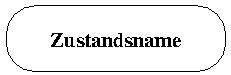
\includegraphics[width=4cm]{uml/img/Zustand}
\fi
\end{minipage}
\begin{minipage}[c]{0.7\linewidth}
Der Name des Zustands ist optional. Zust\"ande ohne Namen
heissen anonyme Zust\"ande und sind alle voneinander verschieden.
Ein benannter Zustand kann dagegen - der besseren Lesbarkeit halber -
mehrmals in das Diagramm eingetragen werden.
\end{minipage}
%
\paragraph{Action}\ \\[2ex]
\begin{minipage}[c]{0.28\linewidth}
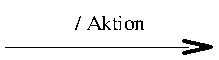
\includegraphics[width=3.5cm]{uml/img/Aktion}
\end{minipage}\hfill
\begin{minipage}[c]{0.7\linewidth}
Mit einem Zustand oder einer Transition k\"onnen Aktionen oder
Aktivit\"aten verbunden sein. \\
\end{minipage}
%
\begin{minipage}[c]{0.28\linewidth}
\ifslides
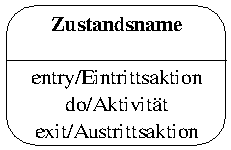
\includegraphics[width=3cm]{uml/img/Zustandsname}
\else
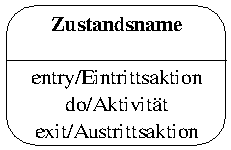
\includegraphics[width=4cm]{uml/img/Zustandsname}
\fi
\end{minipage}
\begin{minipage}[c]{0.7\linewidth}
\paragraph{entry}\ \\[2ex]
\ifslides
Ausführung bei Entritt
\else
Jede Aktion, die als mit dem Eintrittsereignis assoziiert
markiert ist, wird immer dann ausgef\"uhrt, wenn der vorgegebene
Zustand \"uber eine Transition betreten wird. Eine entry-Aktion ist atomar.
\fi
%
\paragraph{exit}\ \\[2ex]
\ifslides
Ausführung beim Verlassen
\else
Die mit dem Austrittsereignis assoziierte Aktion wird immer ausgef\"uhrt,
wenn der Zustand \"uber eine Transition verlassen wird. F\"uhrt eine
Transition in den gleichen Zustand zur\"uck (das wird Transitionsschleife
genannt) und besitzt diese eine Aktion, dann wird die Austrittsaktion
zuerst ausgef\"uhrt, dann die Aktion der Transition und anschliessend
die Eintrittsaktion.
\fi
%
\paragraph{do}\ \\[2ex]
\ifslides
Ausführung während des Zustandes
\else
Eine Aktivit\"at beginnt, wenn das Objekt den Zustand einnimmt und endet,
wenn es den Zustand verl\"asst. Zus\"atzlich k\"onnen weitere interne
Aktionen angegeben werden, die durch bestimmte Ereignisse auftreten k\"onnen.
\fi
\end{minipage}
%
\paragraph{Transition}\ \\[2ex]
\begin{minipage}[c]{0.28\linewidth}
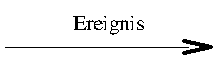
\includegraphics[width=3.5cm]{uml/img/Ereignis}
\end{minipage}
\begin{minipage}[c]{0.7\linewidth}
Eine Transition bzw. ein Zustands\"ubergang verbindet
zwei Zust\"ande. Eine
Transition wird durch ein Ereignis ausgel\"ost und kann
nicht unterbrochen werden.
Man sagt, dass die Transition feuert. Wenn das Ereignis
nicht angegeben wird, handelt
es sich um ein implizites Ereignis.
\end{minipage}
%
\paragraph{Guard condition}\ \\[2ex]
\begin{minipage}[c]{0.28\linewidth}
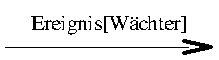
\includegraphics[width=3.5cm]{uml/img/EreignisWaechter}
\end{minipage}
\begin{minipage}[c]{0.7\linewidth}
Eine Transition kann zus\"atzlich mit einem W\"achter versehen werden.
Es handelt sich um einen logischen Ausdruck, der ausgewertet wird,
wenn das zugeh\"orige Ereignis eintritt. Nur wenn die Bedingung des
W\"achters erf\"ullt ist, feuert die Transition.
\end{minipage}
%
\paragraph{Event}\ \\[2ex]
Ein Ereignis kann sein:
\begin{itemize}
\item eine Bedingung, die wahr wird,
\item eine Botschaft (Aufruf einer Methode),
\item eine verstrichene Zeitdauer oder
\item das Eintreten eines bestimmten Zeitpunktes.
\end{itemize}
Tritt ein Ereignis ein und das Objekt befindet sich
nicht in einem Zustand, in dem es darauf reagieren kann,
dann wird das Ereignis ignoriert.

Ein Zustand kann analog der Klasse mit Variablen und Aktivitäten
zusätzlich beschrieben werden:
\begin{center}
\ifslides
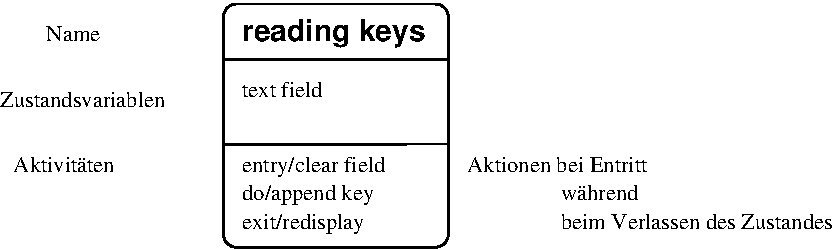
\includegraphics[width=0.7\linewidth]{uml/xfig/uml-state}
\else
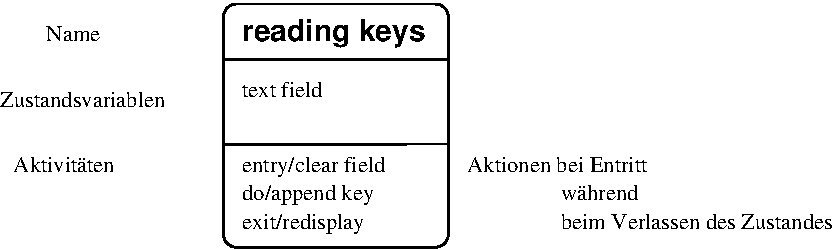
\includegraphics[width=0.9\linewidth]{uml/xfig/uml-state}
\fi
\end{center}
\underline{Vorgehen}
\begin{enumerate}
\item Szenarien entwerfen
\item Ereignisse und betroffene Objekte identifizieren
\item Zustandsdiagramm entwickeln
\end{enumerate}
\newpage
%--------------------------------------------------------------------------
\section{Use-Case Diagram}
\begin{center}
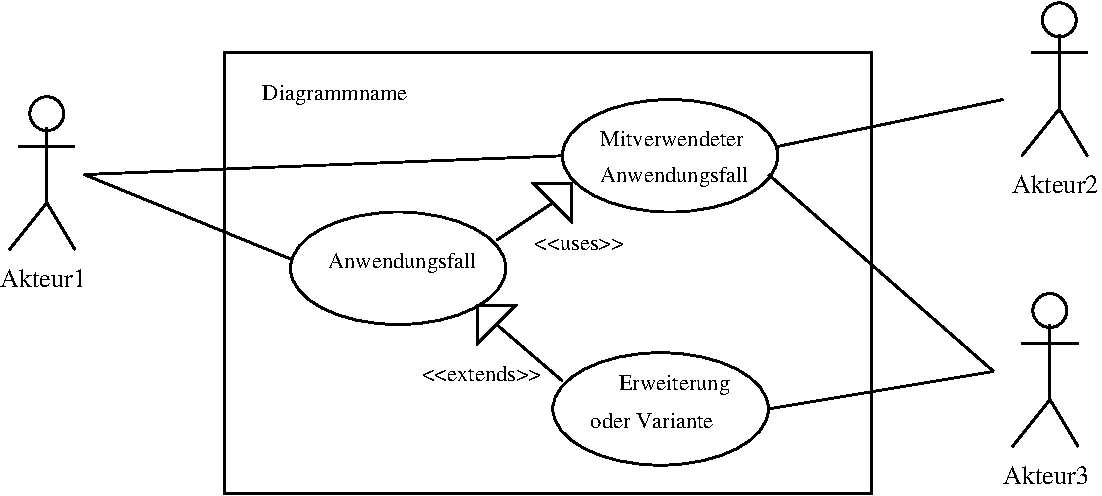
\includegraphics[width=\linewidth]{uml/xfig/uml-usecase}
\end{center}
% Craig Larman UML and Patterns

\ifslides
\newpage
\fi
Ein Anwendungsfall ist die Beschreibung eines Arbeitsablaufes, einer
typischen Interaktion zwischen einem Anwender (Akteur) und dem System.
Hauptsächlicher Zweck der Use-Case-Diagramme ist die allgemeinverständliche
Dokumentation des Anwendungsfachgebietes.\\[2ex]
\underline{Vorgehen}
\begin{enumerate}
\item Arbeitsabläufe (Interaktionen) und Akteure identifizieren
   und beschreiben,
\item Begriffe (Fachausdrücke) des Anwendungsgebietes klären
\item Anwendungsfalldiagramme erstellen
\end{enumerate}
\newpage
%\begin{minipage}[c]{0.38\linewidth}
\ifslides
\begin{center}
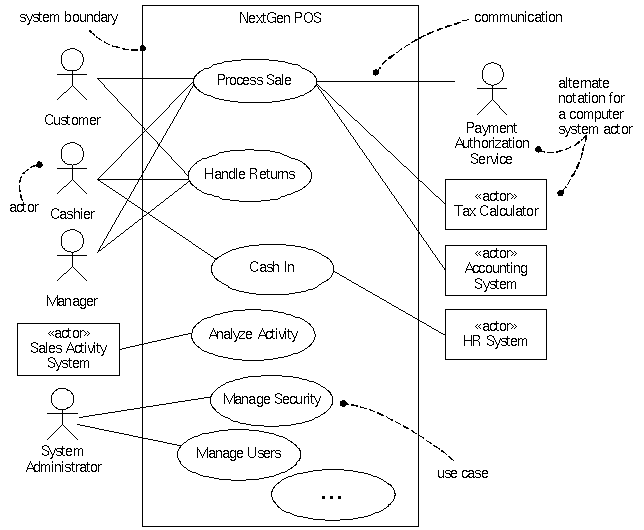
\includegraphics[width=0.8\linewidth]{uml/img/usecase}
\end{center}
\else
\begin{figure}[H]
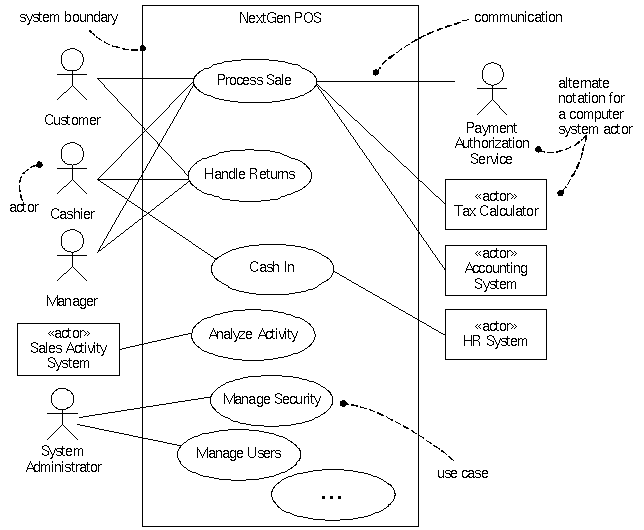
\includegraphics[width=\linewidth]{uml/img/usecase}
\caption{Use-Case eines Point-Of-Sale-Systems (Source: Craig Larman)}
\end{figure}
\fi
%\end{minipage}
%\begin{minipage}[c]{0.6\linewidth}
\emph{Akteure} interagieren mit dem System. Es sind Rollen, die
Benutzer des Systems spielen. Akteure können Personen oder externe
Systeme sein.
%\end{minipage}
%
%\begin{minipage}[c]{0.38\linewidth}
%\includegraphics[width=4.5cm]{uml/img/AnwendungsfallC}
%\end{minipage}
%\begin{minipage}[c]{0.6\linewidth}

Ein \emph{Anwendungsfall} beschreibt ein bestimmtes Verhalten des zu
erstellenden Systems.
%\end{minipage}
%
%\begin{minipage}[c]{0.38\linewidth}
%\includegraphics[width=4.5cm]{uml/img/KommentarC}
%\end{minipage}
%\begin{minipage}[c]{0.6\linewidth}

Einem Anwendungsfall kann ein Kommentar zugeordnet sein.
%\end{minipage}
%
%\begin{minipage}[c]{0.7\linewidth}
%\ifslides
%\includegraphics[width=7.5cm]{uml/img/BeziehungC}
%\else
%\includegraphics[width=9.5cm]{uml/img/BeziehungC}
%\fi
%\end{minipage}
%\begin{minipage}[c]{0.28\linewidth}

Jeder Akteur hat mindestens eine \emph{Beziehung} zu einem Anwendungsfall.

Akteure können auch externe Systeme sein.

%\end{minipage}
%
%\begin{minipage}[c]{0.6\linewidth}
%\includegraphics[width=7.5cm]{uml/img/Beziehung2C}
%\end{minipage}
%\begin{minipage}[c]{0.38\linewidth}

Anwendungsf\"alle k\"onnen nicht nur zu Akteuren,
sondern auch untereinander in \emph{Beziehung} stehen.

%Die \emph{include Beziehung} bedeutet hier, dass jedesmal,
%wenn \texttt{Datei ausw\"ahlen und \"offnen} ausgef\"uhrt wird,
%auch \texttt{Titel und \"Uberschriften in der HTML-Seite lesen} ausgef\"uhrt
%wird.
%\end{minipage}
%
%\begin{minipage}[c]{0.6\linewidth}
%\includegraphics[width=7.5cm]{uml/img/ExtendC}
%\end{minipage}
%\begin{minipage}[c]{0.38\linewidth}
%Der allgemeinere Anwendungsfall \texttt{Einstellungen vornehmen}
% wird spezialisiert durch den Anwendungsfall \texttt{Papierformat w\"ahlen}.
%\end{minipage}\\
%\begin{minipage}[c]{0.58\linewidth}
%\ifslides
%\includegraphics[width=7cm]{uml/img/VerallgemeinerungC}
%\else
%\includegraphics[width=7.5cm]{uml/img/VerallgemeinerungC}
%\fi
%\end{minipage}\hfill
%\begin{minipage}[c]{0.4\linewidth}
%Auch Akteure lassen sich verallgemeinern bzw. spezialisieren: Auch der
%Techniker ist ein Anwender.
%\end{minipage}\\
%--------------------------------------------------------------------------
%\underline{Anwendungsfalldiagramm (Use-Case-Diagram)}
%
%--------------------------------------------------------------------------
% Siehe auch
% http://www.readysetpro.com/whitepapers/usecasetut.html
%--------------------------------------------------------------------------
\newpage
\ifslides
\includegraphics[width=\linewidth]{uml/xfig/kontext-diagramm}
\else
\paragraph{Beispiel Antriebsauslegung}
 Es soll ein Programm erstellt werden, das den
Antriebsprojektierer bei der energie-optimalen
Auswahl von Normmotoren unterst\"utzt. Dabei sollen ihm
nach Eingabe der Projektierungsdaten
verschiedene m\"ogliche Varianten angeboten werden, aus welcher er dann
eine Auswahl treffen kann. Auf Wunsch soll der gew\"ahlte Motor
direkt im Lager bestellt werden k\"onnen. Sofern ein solcher
vorrätig ist, wird vom System ein Lieferauftrag erzeugt, der dem zuständigen
Lagermitarbeiter per E-mail zugeschickt wird. Der Einkauf ist dafür
besorgt, dass die Motordaten stets nachgeführt sind.\\
\vspace{1.5cm}

\includegraphics[width=\linewidth]{uml/xfig/kontext-diagramm}
\fi
%\newpage
%\ifslides
%\begin{center}
%\includegraphics[width=0.7\linewidth]{uml/img/AnwendungsfalldiagrammC}
%\end{center}
%\else
%\paragraph{Beispiel Fotokopierer}
%Der Anwender soll Fotokopien erstellen k\"onnen. Dazu muss er zun\"achst
%das Ger\"at einschalten. Danach muss er Einstellungen vornehmen, und zwar
% zuerst das Papierformat w\"ahlen und dann die gew\"unschte Zahl zu
%erstellender Kopien. Danach ist das Original einzulegen und das Kopieren
%kann gestartet werden. Liegt kein Original vor, wird auch nicht kopiert.
%Der Anwender kann das Kopieren auch jederzeit abbrechen. Der Techniker
%f\"uhrt die Wartung durch, dazu geh\"ort zuerst das Toner auff\"ullen
%und dann die Reinigung des Ger\"ates.
%
%\begin{figure}[H]
%\begin{center}
%\includegraphics[width=\linewidth]{uml/img/AnwendungsfalldiagrammC}
%\caption{Anwendungsfalldiagramm Fotokopierer}
%\end{center}
%\end{figure}
%\fi
%
%--------------------------------------------------------------------------
\section{Package Diagram}
\ifslides
\begin{center}
\includegraphics[width=0.6\linewidth]{uml/img/packages}
\end{center}
\else
\begin{figure}[H]
\includegraphics[width=\linewidth]{uml/img/packages}
\caption{Paketdiagramm (Source: Craig Larman)}
\end{figure}
Mit Paketen werden verschiedene Elemente (meist Klassen) zusammengefasst.
\fi

\section{Activity Diagram}
Das Aktivit\"atsdiagramm (engl. activity diagramm) kombiniert Ideen aus
mehreren Techniken, den
Ereignisdiagrammen (engl. event diagramms) von Jim Odell, der zustandsbasierten
Modellierungstechnik SDL, Workflow-Modellierung sowie Petri-Netzen. Diese
Diagramme sind
insbesondere im Zusammenhang mit Arbeitsvorg\"angen und bei der Beschreibung
von Verhalten mit
parallel ablaufenden Anteilen n\"utzlich.
\paragraph{Beispiel Auftragsbearbeitung}
Der Vorgang beginnt mit dem Erhalt eines Auftrages.
Es wird in der Folge eine Rechnung versandt und
parallel dazu der Auftrag
fertiggestellt. Bei einem Eilauftrag wird \"uber Nacht ausgeliefert,
sonst auf normale Weise.
Sobald die Zahlung erhalten und die Auslieferung geschehen ist,
wird der Auftrag abgeschlossen.
\ifslides
\begin{center}
\includegraphics[width=0.6\linewidth]{uml/img/Aktivitaetsdiagramm}
\end{center}
\else
\begin{figure}[H]
\begin{center}
\includegraphics[width=0.8\linewidth]{uml/img/Aktivitaetsdiagramm}
\caption{Aktivitätsdiagramm}
\end{center}
\end{figure}
\fi
%
\newpage
\paragraph{Aktivit\"at}\ \\[2ex]
\begin{minipage}[c]{0.28\linewidth}
\includegraphics[width=3cm]{uml/img/Aktivitaet}
\end{minipage}
\begin{minipage}[c]{0.7\linewidth}
Eine Aktivit\"at ist ein Zustand, in dem etwas getan wird: entweder ein
Prozess in der realen Welt, wie die Eingabe eines Zeichens, oder die Ausf\"uhrung
einer Softwareroutine, wie der Aufruf einer Methode einer Kasse.
\end{minipage}
%
%\newpage
\paragraph{Verzweigung} (engl. branch)\\[2ex]
\begin{minipage}[c]{0.49\linewidth}
\ifslides
\includegraphics[width=5.8cm]{uml/img/branch}
\else
\includegraphics[width=6.3cm]{uml/img/branch}
\fi
\end{minipage}
\begin{minipage}[c]{0.5\linewidth}
Eine Verzweigung besitzt eine einzelne Eingangstransition
und mehrere bewachte Ausgangstransitionen. Genau eine der
Ausgangstransitionen wird genommen. Deshalb sollten die
W\"achterbedigungen sich wechselseitig ausschliessen.
\end{minipage}
%
\newslide
%\newpage
\paragraph{Zusammenf\"uhrung einer Verzweigung} (engl. merge)\\[2ex]
\begin{minipage}[c]{0.29\linewidth}
\ifslides
\includegraphics[width=3.5cm]{uml/img/merge}
\else
\includegraphics[width=4.2cm]{uml/img/merge}
\fi
\end{minipage}
\begin{minipage}[c]{0.7\linewidth}
Eine Zusammenf\"uhrung besitzt mehrere Eingangstransitionen und
einen einzelnen Ausgang. Eine
Zusammenf\"uhrung markiert das Ende eines durch die Verzweigung
eingeleiteten bedingten Verhaltens.
\end{minipage}

Die Raute f\"ur die Verzweigung und Zusammenf\"uhrung muss
nicht explizit gezeichnet werden. Eine
Aktivit\"at kann wie jeder Zustand mehrere bewachte
 Ausgangstransitionen und mehrere Eingangstransitionen besitzen.
%
\ifslides
\newpage
\fi
\paragraph{Aufspaltung} (engl. fork)\\[2ex]
\begin{minipage}[c]{0.29\linewidth}
\ifslides
\includegraphics[width=3.8cm]{uml/img/fork}
\else
\includegraphics[width=4.2cm]{uml/img/fork}
\fi
\end{minipage}
\begin{minipage}[c]{0.7\linewidth}
Eine Aufspaltung besitzt eine Eingangstransition und
mehrere Ausgangstransitionen. Wird die
Eingangstransition ausgel\"ost, werden alle Ausgangstransitionen
gleichzeitig verfolgt.
\end{minipage}

Das Diagramm sagt aus, dass diese Aktivit\"aten parallel
stattfinden k\"onnen. Das heisst also,
dass die Reihenfolge dieser Aktivit\"aten unwichtig ist.

Flussdiagramme sind normalerweise auf sequentielle Prozesse
beschr\"ankt. Aktivit\"ats\-dia\-gramme
k\"onnen hingegen auch parallele Prozesse modellieren.

Dies ist f\"ur die Modellierung von Gesch\"aftsvorg\"angen
vorteilhaft, da Unternehmen oft
Vorg\"ange mit unn\"otigen Reihenfolgevorschriften aufweisen.
Eine Technik wie diese, die die
Modellierung parallelen Verhaltens erm\"oglicht, tr\"agt dazu bei,
dass die Beteiligten sich
\"uber unn\"otige Reihenfolgebedingungen bewusst werden und
Parallelisierungsm\"oglichkeiten
erkennen k\"onnen. Dies kann die Effizienz und die
Durchlaufzeiten von Gesch\"aftsvorg\"angen
verbessern.
%
\newpage
\paragraph{Zusammenf\"uhrung einer Aufspaltung} (engl. join)\\[2ex]
\begin{minipage}[c]{0.29\linewidth}
\ifslides
\includegraphics[width=3.8cm]{uml/img/join}
\else
\includegraphics[width=4.2cm]{uml/img/join}
\fi
\end{minipage}
\begin{minipage}[c]{0.7\linewidth}
Bei parallelen Verhalten muss man die Vorg\"ange untereinander
synchronisieren. Dies zeigen wir
mit dem Join an. Bei einem Join wird die Ausgangstransition nur
beschritten, wenn alle Zust\"ande
an den Eingangstransitionen ihre Aktivit\"aten abgeschlossen haben.
\end{minipage}

Aufspaltung und Joins m\"ussen paarweise zusammen auftreten.
Im einfachsten Fall bedeutet dies,
dass alle durch eine Aufspaltung erzeugten Threads durch ein
Join wieder zusammengef\"uhrt werden
m\"ussen. (Diese Regel r\"uhrt daher, dass das Aktivit\"atsdiagramm
derzeit eine Form des
Zustandsdiagramms ist).
%
\ifslides
\newpage
\fi
\paragraph{Bedingter Thread}\ \\[2ex]
\begin{minipage}[c]{0.49\linewidth}
\ifslides
\includegraphics[width=5.8cm]{uml/img/thread}
\else
\includegraphics[width=6.2cm]{uml/img/thread}
\fi
\end{minipage}
\begin{minipage}[c]{0.5\linewidth}
Zu der Regel, dass vor dem Betreten des Joins alle seine
Einganszust\"ande beendet sein m\"ussen,
existiert eine Ausnahme. Man kann dem aus einer Aufspaltung
hervorgehenden Thread eine Bedingung
hinzuf\"ugen. Das Ergebnis ist ein bedingter Thread. Wird
w\"ahrend der Ausf\"uhrung die Bedingung
eines bedingten Threads zu falsch ausgewertet, wird dieser
Thread in bezug auf den Join als
abgeschlossen betrachtet.
\end{minipage}
%
\ifslides
\newpage
\fi
\paragraph{Dynamische Nebenl\"aufigkeit}\ \\[2ex]
\begin{minipage}[c]{0.29\linewidth}
\includegraphics[width=3cm]{uml/img/Nebenlaeufigkeit}
\end{minipage}
\begin{minipage}[c]{0.7\linewidth}
Die dynamische Nebenl\"aufigkeit erm\"oglicht das Notieren von
Iterationen, ohne explizit eine
Schleife konstruieren zu m\"ussen.
\end{minipage}
%
\paragraph{Veranwortlichkeitsbereich} (engl. swimlanes)\\[2ex]
Wenn man mit Verantwortlichkeitsbereichen arbeiten will,
können die Aktivit\"ats\-dia\-gramme in
vertikal verlaufende Zonen angeordnet werden. Jeder
Bereich repr\"asentiert die Verantwortlichkeiten einer bestimmten Klasse.
%
%------------------------------------------------------------------------
\section{Exercise}
\begin{enumerate}
\item Create a use case diagram for the Web Application component.
Try to describe as much information as needed. The web application will
be used to search and retrieve data over the REST component.
\end{enumerate}

%\newpage
\section{Software and further Informations}
\begin{itemize}
\item Der UML-Standard: \href{http://www.uml.org/}{http://www.uml.org/}
%\item Eine umfassende Liste mit UML-Tools:
%  \href{http://www.jeckle.de/umltools.htm}{www.jeckle.de/umltools.htm}
%\item Notationsübersicht und Glossar in Deutsch:
%  \href{http://www.oose.de/uml.htm}{www.oose.de/uml.htm}
%\item UML-Tutorial: \href{http://ivs.cs.uni-magdeburg.de/~dumke/UML/index.htm}
%                  {ivs.cs.uni-magdeburg.de/\~dumke/UML/index.htm}
\item UMLGraph: deklaratives Zeichnen von UML-Diagrammen
   \href{http://www.spinellis.gr/umlgraph}{www.spinellis.gr/umlgraph}
%\item LightUML: Eclipse-Plugin zur Generierung von UML-Diagrammen
%aus Java-Klassen
%  \href{http://lightuml.sourceforge.net/}{lightuml.sourceforge.net}
%\item Craig Larman: Autor des UML-Bestsellers ``Applying UML and
%  Patterns: An Introduction to Object-Oriented Analysis and Design and
%  Iterative Development''
%\href{http://www.craiglarman.com/}{www.craiglarman.com/}
%
%
%    http://se.cs.uni-magdeburg.de/tutorial/UML2/Einfuehrung.htm
%    http://dn.codegear.com/article/31863
%    http://uml-tutorials.trireme.com/
%    http://www.jeckle.de/files/umltutorial.pdf
%
%
\end{itemize}
%%% Local Variables:
%%% mode: latex
%%% TeX-master: t
%%% End:
